% Workstream structural: results. Numbers are macros from the AUTO block of method_structural.tex;
% tables are generated by `python -m albert.research.flb_structural run latex` (data/research/flb_structural/).

We ask how much of the longshot overpricing each explanation of \cref{sec:framework} accounts for, using the
methods of \cref{sec:method-structural}. The sample is the final panel of \cref{sec:res-xs}: \sdQuotes{} pre-event
quotes on \sdMarkets{} markets in \sdEvents{} events, with \sdLsSides{} longshot side observations. Quantities are
in cents per contract at the calibration level, because pooled returns per dollar on longshots rest on a few large
wins (\cref{sec:res-flow}). Supporting tables and figures are in \cref{app:structural}.

\subsubsection{Mechanical frictions}\label{sec:res-structural-band}

\Cref{tab:structural-band,fig:structural-band} decompose the longshot gap as in~\eqref{eq:structural-decomp}.
\begin{itemize}
  \item \emph{Size of the gap.} Longshot sides cost \sdLsPrice\cents{} at the mid and win \sdLsWin\% of the time,
  a gap of \sdLsGross\cents{} per contract ($t=\sdLsGrossT$).
  \item \emph{Cost of selling as a taker.} It is \sdLsBand\cents:
  \begin{itemize}
    \item \sdLsFloor{} of half-spread at the tick floor;
    \item \sdLsSpread{} of other half-spread;
    \item \sdLsFee{} of fees;
    \item \sdLsCap{} of capital at 5\% a year.
  \end{itemize}
  \item \emph{Residual.} It is $\bar R=\sdLsResid\cents$ ($t=\sdLsResidT$). Market-weighted, the mispricing lies
  inside the taker band in every price bucket, as in \cref{tab:xs-limits}. In no group is the residual
  significantly positive.
  \item \emph{Sides with a bid.} Where a taker sale is possible at all, the residual is \sdRobBidResid\cents{}
  ($t=\sdRobBidResidT$). This is the per-contract counterpart of taking the other side of longshots in
  \cref{tab:xs-limits}.
  \item \emph{Short leads.} At leads of a day or less, the gap sits at the edge of the band (residuals of
  \sdLeadOneHResid, \sdLeadSixHResid{} and \sdLeadOneDResid\cents).
\end{itemize}

Frictions thus explain why takers do not trade the bias away, but not where it comes from.
\begin{enumerate}
  \item \emph{The floor explains the cheapest bucket only.} The floor's half-spread is \sdBOneFloorShare\% of the
  1--2\cents{} gap. \Cref{tab:xs-limits} finds less because it counts the realised loss of floor quotes. Across all
  longshots, the floor is \sdLsFloorShare\% of the gap. On the 0.1\cents{} grid, whose floor is ten times lower
  (\sdSubCentBN{} sides, \sdSubCentBClusters{} events), the 1--2\cents{} gap is \sdSubCentBGross\cents{}, against
  \sdOneCentBGross\cents{} on the 1\cents{} grid, with a residual of \sdSubCentBResid\cents{} ($t=\sdSubCentBResidT$).
  \item \emph{The bias does not grow with the horizon.} Capital costs at most \sdLeadThirtyDCap\cents{} at 30 days.
  Within price buckets, the gap \emph{falls} by \sdHzGross\cents{} per unit of log lead ($t=\sdHzGrossT$), and the
  residual by \sdHzResid{} ($t=\sdHzResidT$). The raw gap is larger at 30 days (\sdLeadThirtyDGross{} against
  \sdLeadOneHGross\cents) because longshots quoted that far ahead are dearer (\sdLeadThirtyDPrice{} against
  \sdLeadOneHPrice\cents{} at the mid). \Cref{hyp:mech} and \citet{pageclemen2013}
  predict growth with the horizon.
  \item \emph{The cost of capital is immaterial.} The residual is \sdRhoZeroResid\cents{} at $\rho=0$ and
  \sdRhoTenResid\cents{} at $\rho=10\%$.
  \item \emph{Where the volume is, the bias exceeds the band.} Volume-weighted, the gap is \sdLsVolGross\cents{}
  but the band only \sdLsVolBand\cents, because active markets have tight spreads. The residual is
  \sdLsVolResid\cents{} ($t=\sdLsVolResidT$).
  \item \emph{Makers could earn the gap.} Selling at the ask would earn $\bar R^{mk}=\sdLsResidMk\cents$
  ($t=\sdLsResidMkT$). This is an upper bound that ignores adverse selection, consistent with \cref{sec:res-flow}.
\end{enumerate}

\begin{figure}[!htbp]
\centering
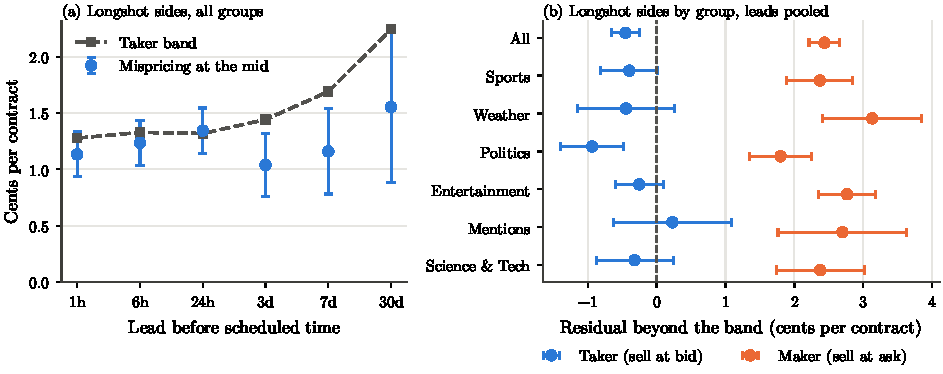
\includegraphics[width=\textwidth]{figures/fig_structural_band.pdf}
\caption{The longshot mispricing and the no-arbitrage band. Left: price at the mid minus realised win rate of
longshot sides ($\q\le10\cents$) by lead, against the taker band (tick floor, half-spread, fee and capital at
$\rho=5\%$). Right: the residual beyond the band, the mean profit per contract of selling longshots at the bid
(taker) or at the ask (maker, an upper bound), by group with leads pooled. Market-weighted; 95\% confidence
intervals clustered by event.}\label{fig:structural-band}
\end{figure}

% BEGIN AUTO:tab-band
\begin{table}[!htbp]
\centering
\begin{threeparttable}
\caption{Longshot mispricing and the no-arbitrage band}\label{tab:structural-band}
\scriptsize
\setlength{\tabcolsep}{3pt}
\begin{tabular}{@{}lrrrrrrrrrrr@{}}
\toprule
 & & & & Gross & \multicolumn{4}{c}{Band components} & Residual & Maker & In band \\
\cmidrule(lr){6-9}
Cell & Sides & Events & $\bar\q$ & $\bar\q-\bar\won$ & Floor & Half-spr. & Fee & Capital & $\bar R$ & $\bar R^{mk}$ & (\%) \\
\midrule
% source: data/research/flb_structural/band_cells.csv
All longshots & 40{,}552 & 3{,}091 & 2.54 & 1.07 (10.0) & 0.18 & 1.23 & 0.07 & 0.04 & $-$0.45 ($-$4.3) & 2.44 (21.3) & 100 \\
\multicolumn{12}{@{}l}{\emph{By lead, all groups}} \\
\quad 1h & 9{,}847 & 2{,}690 & 2.05 & 1.13 (11.2) & 0.23 & 0.99 & 0.05 & 0.00 & $-$0.14 ($-$1.5) & 2.35 (21.7) & 100 \\
\quad 6h & 9{,}721 & 2{,}633 & 2.17 & 1.24 (12.2) & 0.21 & 1.06 & 0.06 & 0.00 & $-$0.09 ($-$0.9) & 2.49 (23.1) & 100 \\
\quad 24h & 8{,}025 & 1{,}962 & 2.10 & 1.34 (13.1) & 0.20 & 1.04 & 0.06 & 0.01 & 0.03 (0.3) & 2.57 (22.9) & 98 \\
\quad 3d & 7{,}056 & 1{,}742 & 2.44 & 1.04 (7.3) & 0.17 & 1.16 & 0.07 & 0.04 & $-$0.40 ($-$2.9) & 2.32 (15.1) & 100 \\
\quad 7d & 4{,}149 & 1{,}180 & 2.56 & 1.16 (6.0) & 0.15 & 1.38 & 0.07 & 0.09 & $-$0.53 ($-$2.8) & 2.59 (12.5) & 100 \\
\quad 30d & 1{,}754 & 670 & 3.38 & 1.55 (4.5) & 0.09 & 1.64 & 0.11 & 0.40 & $-$0.69 ($-$2.0) & 2.89 (8.0) & 100 \\
\multicolumn{12}{@{}l}{\emph{By group, leads pooled}} \\
\quad Sports & 9{,}108 & 502 & 2.29 & 1.07 (4.9) & 0.22 & 1.14 & 0.06 & 0.04 & $-$0.40 ($-$1.9) & 2.37 (9.7) & 100 \\
\quad Weather & 3{,}905 & 721 & 3.46 & 1.42 (4.0) & 0.11 & 1.62 & 0.12 & 0.02 & $-$0.44 ($-$1.2) & 3.13 (8.6) & 100 \\
\quad Politics & 11{,}768 & 835 & 2.51 & 0.51 (2.2) & 0.15 & 1.17 & 0.08 & 0.04 & $-$0.94 ($-$4.0) & 1.80 (7.8) & 100 \\
\quad Entertainment & 8{,}939 & 494 & 2.22 & 1.31 (7.1) & 0.19 & 1.30 & 0.05 & 0.03 & $-$0.25 ($-$1.4) & 2.76 (13.2) & 100 \\
\quad Mentions & 1{,}918 & 91 & 3.22 & 1.55 (3.5) & 0.20 & 0.96 & 0.14 & 0.02 & 0.23 (0.5) & 2.70 (5.7) & 85 \\
\quad Science \& Tech & 4{,}572 & 401 & 2.30 & 1.12 (3.8) & 0.18 & 1.14 & 0.07 & 0.05 & $-$0.32 ($-$1.1) & 2.37 (7.3) & 100 \\
\bottomrule
\end{tabular}
\begin{tablenotes}\footnotesize
\item Side observations with $\q\le10\cents$ at the mid, pre-event quotes. All entries in cents per contract. Gross: price at the mid minus the realised win rate. The band components (\cref{eq:structural-decomp}) are the half-spread of sides pinned at the tick floor (Floor), the half-spread of other sides, the taker fee and the capital cost at $\rho=5\%$ a year over the lead. $\bar R$: residual beyond the taker band, the mean net profit per contract of selling the side at its bid; $\bar R^{mk}$: selling at its ask as a maker (an upper bound: no adverse selection). In band: share of the gross mispricing the taker band covers, $\min(\text{band},\text{gross})/\text{gross}$. Market-weighted (each market once per cell; within a lead, equal weights). Cells by price bucket and structure are in \cref{tab:structural-band-groups,tab:structural-band-robust}; the band per bucket agrees with \cref{tab:xs-limits}. $t$-statistics clustered by event in parentheses.
\end{tablenotes}
\end{threeparttable}
\end{table}
% END AUTO:tab-band

\subsubsection{Probability weighting}\label{sec:res-structural-weighting}

In \cref{tab:structural-weighting}, the LLO curvature is $\gamma=1/\beta$ for the slope $\beta$ of
\cref{tab:xs-group}, estimated on the identical sample.
\begin{itemize}
  \item \emph{Pooled.} $\gamma=\sdAllGamma$ (standard error \sdAllGammaSe; $t_{\gamma<1}=\sdAllGammaT$), and the
  Prelec curvature is also \sdAllPrGamma. Both overweight small probabilities, with near-neutral elevation
  ($\delta=\sdAllDelta$ and \sdAllPrDelta).
  \item \emph{Groups.} $\gamma$ is below one in \sdGammaBelowOne{} of \sdNGroups{} groups (\sdGammaMin--\sdGammaMax).
  A common $\gamma$ is not rejected market-weighted ($p=\sdWaldGroupP$). It is rejected volume-weighted
  ($p=\sdWaldGroupVolP$), where the distortion is stronger ($\gamma=\sdAllVolGamma$).
  \item \emph{Leads and halves.} Across leads $\gamma$ ranges from \sdLeadGammaMin{} to \sdLeadGammaMax{}
  ($p=\sdWaldLeadP$). It is \sdHalfFirstGamma{} and \sdHalfSecondGamma{} in the two halves.
  \item \emph{Out of sample.} Fitted on one half of the months and scored on the other, pooled LLO improves the log
  score of face-value prices by only \sdOosFsLlo{} ($t=\sdOosFsLloT$) and \sdOosSfLlo{} milli-nats per quote, and
  Prelec by \sdOosFsPrelec{} and \sdOosSfPrelec. The log loss itself is \sdOosFsCalLs{} nats. A constant YES shift
  lowers the score (\sdOosFsShift, $t=\sdOosFsShiftT$). Group-specific LLO is worse than pooled LLO by
  \sdOosFsGroupVsPooled{} ($t=\sdOosFsGroupVsPooledT$) and \sdOosSfGroupVsPooled{} ($t=\sdOosSfGroupVsPooledT$).
\end{itemize}
One mild inverse-S function thus describes all categories. It is precisely estimated but small next to the
information in prices.

% BEGIN AUTO:tab-weighting
\begin{table}[!htbp]
\centering
\begin{threeparttable}
\caption{Probability weighting: fitted functions, equality tests and forecasts}\label{tab:structural-weighting}
\scriptsize
\setlength{\tabcolsep}{3.5pt}
\begin{tabular}{@{}lrrrrrrrrr@{}}
\toprule
 & & & \multicolumn{3}{c}{LLO} & \multicolumn{2}{c}{Prelec} & \multicolumn{2}{c}{$\Delta\log L$} \\
\cmidrule(lr){4-6}\cmidrule(lr){7-8}\cmidrule(l){9-10}
Group & Quotes & Events & $\gamma$ & $\delta$ & $t_{\gamma<1}$ & $\gamma$ & $\delta$ & LLO & Prelec \\
\midrule
% source: data/research/flb_structural/weighting_fits.csv, weighting_insample.csv, weighting_oos.csv, summary.json:weighting.wald
\multicolumn{10}{@{}l}{\emph{Panel A. Fitted weighting functions}} \\
All groups & 61{,}992 & 4{,}770 & 0.89 (0.016) & $-$0.06 (0.029) & 7.4 & 0.89 (0.016) & 1.01 (0.016) & 1.4 & 1.6 \\
Sports & 18{,}303 & 1{,}521 & 0.91 (0.031) & $-$0.04 (0.047) & 2.9 & 0.90 (0.027) & 1.00 (0.027) & 0.8 & 1.2 \\
Weather & 6{,}796 & 1{,}065 & 0.87 (0.040) & $-$0.10 (0.047) & 3.3 & 0.89 (0.039) & 1.02 (0.022) & 1.6 & 1.6 \\
Politics & 15{,}774 & 968 & 0.93 (0.036) & $-$0.07 (0.065) & 1.9 & 0.93 (0.035) & 1.03 (0.032) & 0.4 & 0.5 \\
Entertainment & 10{,}424 & 530 & 0.80 (0.034) & 0.04 (0.076) & 6.0 & 0.85 (0.035) & 0.97 (0.041) & 5.1 & 5.0 \\
Mentions & 4{,}743 & 103 & 0.89 (0.049) & $-$0.03 (0.106) & 2.3 & 0.88 (0.052) & 0.99 (0.060) & 1.5 & 2.0 \\
Science \& Tech & 5{,}472 & 510 & 0.85 (0.049) & $-$0.17 (0.141) & 3.0 & 0.84 (0.052) & 1.08 (0.083) & 3.2 & 3.6 \\
\midrule
\multicolumn{10}{@{}l}{\emph{Panel B. Equal slopes ($\gamma$) across cells: Wald tests}} \\
\multicolumn{3}{@{}l}{Groups} & \multicolumn{7}{l}{$\chi^2_{5}=8.6$, $p=0.127$, 4{,}697 events} \\
\multicolumn{3}{@{}l}{Groups, $\gamma$ and $\delta$} & \multicolumn{7}{l}{$\chi^2_{10}=16.6$, $p=0.084$, 4{,}697 events} \\
\multicolumn{3}{@{}l}{Structures} & \multicolumn{7}{l}{$\chi^2_{3}=7.5$, $p=0.057$, 4{,}770 events} \\
\multicolumn{3}{@{}l}{Leads} & \multicolumn{7}{l}{$\chi^2_{5}=12.1$, $p=0.033$, 4{,}770 events} \\
\multicolumn{3}{@{}l}{Groups, volume-weighted} & \multicolumn{7}{l}{$\chi^2_{5}=12.8$, $p=0.026$, 4{,}357 events} \\
\midrule
\multicolumn{10}{@{}l}{\emph{Panel C. Out-of-sample log score against calibrated prices (milli-nats per quote)}} \\
\multicolumn{3}{@{}l}{Constant shift} & \multicolumn{7}{l}{first $\to$ second half: $-$1.32 ($-$2.9); second $\to$ first: $-$0.73 ($-$4.4)} \\
\multicolumn{3}{@{}l}{LLO, pooled} & \multicolumn{7}{l}{first $\to$ second half: 0.46 (0.9); second $\to$ first: 0.04 (0.1)} \\
\multicolumn{3}{@{}l}{Prelec, pooled} & \multicolumn{7}{l}{first $\to$ second half: 0.75 (1.7); second $\to$ first: 0.19 (0.3)} \\
\multicolumn{3}{@{}l}{LLO, by group} & \multicolumn{7}{l}{first $\to$ second half: $-$2.65 ($-$2.3); second $\to$ first: $-$1.79 ($-$1.6)} \\
\bottomrule
\end{tabular}
\begin{tablenotes}\footnotesize
\item YES sides of pre-event quotes, market-weighted. LLO: $\operatorname{logit}\q=\delta+\gamma\operatorname{logit}\pi$, estimated as~\eqref{eq:logit} with $\gamma=1/\beta$ and $\delta=-\alpha/\beta$. Prelec: $\q=\exp(-\delta(-\ln\pi)^\gamma)$. Maximum likelihood on outcomes; standard errors in parentheses clustered by event (delta method for $\gamma$, $\delta$). $\Delta\log L$: in-sample gain in mean log likelihood over calibrated prices, milli-nats per market. Panel B: cluster-robust Wald tests from one fully interacted logit. Panel C: models fitted on one half of the months and scored on the other; differences against $\Prob(y=1)=\q$ with event-clustered $t$ in parentheses.
\end{tablenotes}
\end{threeparttable}
\end{table}
% END AUTO:tab-weighting

\subsubsection{Insiders}\label{sec:res-structural-shin}

\Cref{tab:structural-shin} extends \cref{tab:xs-multi} to two-leg events and partition ladders, by group and
lead. Of \sdShinAllEventLeads{} event-leads, \sdShinIncomplete{} miss a quote on some leg and \sdShinNotOneYes{} lack
exactly one winner. That leaves \sdShinEventLeads{} on \sdShinUnits{} events. The asks sum to less than one in
\sdShinAskBelow{} of them and the mids in \sdShinMidBelow. Mentions events are not partitions.
\begin{itemize}
  \item \emph{The overround restates the spread.} $\shinz$ from the asks averages \sdShinAllZask, and from the mids
  \sdShinAllZmid. It rises by \sdZregSpread{} per cent of half-spread ($t=\sdZregSpreadT$; $R^2=\sdZregRsq$ with leg
  count). Given the spread, it is higher in the information groups by \sdZregInfo{} ($t=\sdZregInfoT$), small
  against its mean of \sdShinAllZask.
  \item \emph{The shading the outcomes require.} Fitted to outcomes, $\hat\shinz=\sdShinAllZml$
  [\sdShinAllZmlLo, \sdShinAllZmlHi], more than twice the margin's $\shinz$. It is \sdZmlInfo{} in the information
  groups and \sdZmlPublic{} in Sports and Weather (difference \sdZmlDiff, [\sdZmlDiffLo, \sdZmlDiffHi]). Politics
  needs the least of any group (\sdShinPoliticsZml).
  \item \emph{Forecasts} (\cref{tab:structural-shin-forecasts}). Longshot legs are overpriced by \sdLsAllMid\cents{}
  at the mid ($t=\sdLsAllMidT$), \sdLsAllNorm{} after normalisation and \sdLsAllShinAsk{} after Shin's correction from
  the asks. Shin beats the normalised asks by \sdScAllShinAsk{} milli-nats per leg ($t=\sdScAllShinAskT$), as
  \citet{strumbelj2014} found for bookmakers, but it does so by undoing the spread. A $\shinz$ fitted on the first
  half shrinks the second-half gap from \sdLsTestMid{} to \sdLsTestShinFit\cents{} ($t=\sdLsTestShinFitT$), acting
  as a calibration curve like LLO.
  \item \emph{Overpricing and $\shinz$.} Longshot overpricing rises with an event's $\shinz$ from the asks
  (\sdLsOnZ{} cents per unit, $t=\sdLsOnZT$). Since that $\shinz$ mostly measures the spread, the band predicts the
  same.
\end{itemize}

% BEGIN AUTO:tab-shin
\begin{table}[!htbp]
\centering
\begin{threeparttable}
\caption{Shin's insider share in events whose legs partition the outcomes}\label{tab:structural-shin}
\scriptsize
\setlength{\tabcolsep}{2.8pt}
\begin{tabular}{@{}lrrrrrrrr@{}}
\toprule
 & Event- & & Legs & $\sum a-1$ & $\sum p-1$ & $\shinz$ from & $\shinz$ from & $\shinz$ fitted \\
Sample & leads & Events & (med.) & (\%) & (\%) & asks & mids & to outcomes [95\% CI] \\
\midrule
% source: data/research/flb_structural/shin_cells.csv, summary.json:shin.info_vs_public
All partition events & 3{,}955 & 1{,}421 & 2 & 7.8 (33.0) & 1.3 (12.8) & 0.030 (0.0005) & 0.004 & 0.080 [0.020, 0.130] \\
\quad Two-leg events & 2{,}009 & 740 & 2 & 3.0 (40.6) & $-$0.2 ($-$4.0) & 0.032 (0.0008) & 0.003 & 0.025 [0.005, 0.095] \\
\quad Multi-outcome events & 1{,}289 & 381 & 4 & 10.1 (17.1) & 2.2 (7.6) & 0.026 (0.0008) & 0.005 & 0.095 [0.025, 0.245] \\
\quad Partition ladders & 657 & 300 & 9 & 16.7 (38.3) & 3.9 (16.3) & 0.030 (0.0008) & 0.008 & 0.105 [0.005, 0.225] \\
\quad Sports & 2{,}373 & 916 & 2 & 4.7 (20.7) & 0.3 (2.6) & 0.030 (0.0007) & 0.003 & 0.060 [0.020, 0.125] \\
\quad Weather & 237 & 139 & 6 & 15.5 (25.5) & 4.1 (11.4) & 0.034 (0.0014) & 0.010 & 0.110 [0.020, 0.420] \\
\quad Politics & 1{,}011 & 280 & 6 & 12.6 (23.3) & 2.6 (12.3) & 0.028 (0.0008) & 0.005 & 0.025 [0.005, 0.165] \\
\quad Entertainment & 120 & 42 & 8 & 17.9 (8.2) & 6.3 (5.8) & 0.036 (0.0034) & 0.010 & 0.070 [0.005, 0.230] \\
\quad Science \& Tech & 214 & 44 & 7 & 7.6 (5.4) & 1.8 (2.3) & 0.018 (0.0019) & 0.005 & 0.195 [0.090, 0.600] \\
\quad Information minus public & & & & & & $-$0.003 & & 0.015 [$-$0.110, 0.090] \\
\bottomrule
\end{tabular}
\begin{tablenotes}\footnotesize
\item Mutually exclusive events (Kalshi flag) and strike ladders that partition the outcome space, at leads where every leg has a usable quote and exactly one leg settles YES. $a$, $p$: YES ask and mid. $\shinz$ from asks or mids solves~\eqref{eq:shin} ($\shinz=0$ when the prices sum to at most one). Fitted $\shinz$: the value on a grid over $[0,0.6]$ that maximises the log score of the winning leg, with the scale chosen so that probabilities sum to one; 95\% event-bootstrap interval. Each event weighs one across its leads; \cref{tab:xs-multi} weights event-leads equally, hence the small differences in the multi-outcome row. Information groups: Politics, Entertainment, Mentions, Science \& Tech; public: Sports, Weather. Standard errors (of $\shinz$) or $t$-statistics (of the overrounds) clustered by event in parentheses.
\end{tablenotes}
\end{threeparttable}
\end{table}
% END AUTO:tab-shin

\subsubsection{Belief dispersion}\label{sec:res-structural-beliefs}

The slope interactions of~\eqref{eq:structural-interact} are in \cref{tab:structural-beliefs,fig:structural-beliefs}.
\begin{itemize}
  \item \emph{Number of outcomes.} More outcomes steepen the slope by \sdPoolLogOutcomes{} per standard deviation
  ($t=\sdPoolLogOutcomesT$; within groups \sdWithinLogOutcomes, $t=\sdWithinLogOutcomesT$). This is the sign
  \cref{hyp:beliefs} predicts, but not significant.
  \item \emph{Turnover.} Turnover flattens the slope (\sdPoolTurnover, $t=\sdPoolTurnoverT$). The interaction is
  positive in only \sdSignTurnoverPos{} of \sdSignTurnoverOf{} groups.
  \item \emph{Forecast anchor.} The anchor interaction is \sdPoolAnchored{} ($t=\sdPoolAnchoredT$), and it flips
  sign between halves (\sdHalfFirstAnchored{} and \sdHalfSecondAnchored).
  \item \emph{Horizon and spread.} Longer horizons flatten the slope (\sdPoolLogLead, $t=\sdPoolLogLeadT$). Wider
  spreads leave the slope unchanged but raise the longshot gap in cents (\sdLsWSpreadC, $t=\sdLsWSpreadCT$), as the
  band predicts.
\end{itemize}

\subsubsection{Synthesis}\label{sec:res-structural-synthesis}

\Cref{tab:structural-scorecard-groups} summarises the evidence by group; \cref{tab:structural-scorecard} lists every
prediction tested.

% BEGIN AUTO:tab-scorecard-groups
\begin{table}[!htbp]
\centering
\begin{threeparttable}
\caption{The evidence by group}\label{tab:structural-scorecard-groups}
\scriptsize
\setlength{\tabcolsep}{3.5pt}
\begin{tabular}{@{}lrrrrr@{}}
\toprule
 & \multicolumn{2}{c}{\Cref{hyp:mech}: band} & \Cref{hyp:pref}: weighting & \Cref{hyp:info}: insiders & \Cref{hyp:beliefs}: dispersion \\
\cmidrule(lr){2-3}
Group & Residual $\bar R$ (\cents) & In band (\%) & $\gamma$ ($t_{\gamma<1}$) & fitted $\shinz$ [95\% CI] & Turnover \\
\midrule
% source: data/research/flb_structural/scorecard.csv
All groups & $+$ $-$0.45 ($-$4.3) & 100 & $+$ 0.89 (7.4) &  0.080 [0.02, 0.13] & $0$ $-$0.043 ($-$1.5) \\
Sports & $+$ $-$0.40 ($-$1.9) & 100 & $+$ 0.91 (2.9) & $-$ 0.060 [0.02, 0.12] & $0$ 0.025 (0.6) \\
Weather & $+$ $-$0.44 ($-$1.2) & 100 & $+$ 0.87 (3.3) & $-$ 0.110 [0.02, 0.42] & $0$ $-$0.054 ($-$0.4) \\
Politics & $+$ $-$0.94 ($-$4.0) & 100 & $0$ 0.93 (1.9) & $+$ 0.025 [0.01, 0.17] & $-$ $-$0.127 ($-$2.7) \\
Entertainment & $+$ $-$0.25 ($-$1.4) & 100 & $+$ 0.80 (6.0) & $+$ 0.070 [0.01, 0.23] & $0$ $-$0.101 ($-$1.8) \\
Mentions & $+$ 0.23 (0.5) & 85 & $+$ 0.89 (2.3) & -- & $0$ $-$0.107 ($-$1.7) \\
Science \& Tech & $+$ $-$0.32 ($-$1.1) & 100 & $+$ 0.85 (3.0) & $+$ 0.195 [0.09, 0.60] & $0$ $-$0.088 ($-$1.3) \\
\bottomrule
\end{tabular}
\begin{tablenotes}\footnotesize
\item Mark: $+$ consistent with the hypothesis's prediction for the group, $-$ inconsistent, $0$ inconclusive. \Cref{hyp:mech}: $+$ when the longshot residual beyond the taker band is not significantly positive. \Cref{hyp:pref}: $+$ when $\gamma<1$ significantly. \Cref{hyp:info}: in Politics, Entertainment, Mentions and Science \& Tech $+$ when the interval for the fitted $\shinz$ excludes zero; in Sports and Weather, where outcomes are public, $+$ when it includes zero and $-$ when it does not. \Cref{hyp:beliefs}: sign and significance of the turnover interaction (within-group slopes for all groups). Sources and clustering as in \cref{tab:structural-band,tab:structural-weighting,tab:structural-shin,tab:structural-beliefs}.
\end{tablenotes}
\end{threeparttable}
\end{table}
% END AUTO:tab-scorecard-groups

\Cref{tab:structural-decomp} applies each explanation's map from prices to probabilities to the second-half
longshot gap of \sdCfGross\cents.
\begin{itemize}
  \item The taker band covers \sdCfBandShare\% of the gap.
  \item LLO fitted on the first half removes \sdCfLloShare\% (residual \sdCfLloResid\cents, $t=\sdCfLloResidT$).
  Prelec removes \sdCfPrelecShare\%, and group-specific LLO \sdCfLloGroupShare\%.
  \item In partition events, normalisation removes \sdCfNormShare\%, Shin with the margin's $\shinz$
  \sdCfShinAskShare\%, and Shin with a fitted $\shinz$ \sdCfShinFitShare\%.
\end{itemize}
The shares are not additive. The band measures what frictions \emph{allow}; the fitted maps measure what a
calibration curve \emph{describes}.

Prices and outcomes cannot separate four things:
\begin{itemize}
  \item risk-love from probability weighting, which needs bet sizes or exotic bets \citep{snowbergwolfers2010};
  \item weighting from heterogeneous beliefs, since both yield a monotone calibration curve that LLO fits by
  construction \citep{gandhi2015,manski2006};
  \item insiders from the spread, which itself prices informed trading \citep{glostenmilgrom1985};
  \item the true cost of capital.
\end{itemize}
We therefore report no variance decomposition.

\paragraph{Summary of verdicts.}
\begin{enumerate}
  \item \emph{Mechanical (\cref{hyp:mech}): \sdVerdictOne{} (\sdPassedOne{} predictions hold).} Spreads, fees and
  the tick floor explain why the bias survives: market-weighted, it is no larger than the cost of selling it as a
  taker in any group. They do not explain where it comes from. It falls rather than grows with the horizon, a
  finer tick does not remove it, and volume-weighted it exceeds the band.
  \item \emph{Preference (\cref{hyp:pref}): \sdVerdictTwo{} (\sdPassedTwo).} Prices behave as if traders weight
  probabilities with one mild inverse-S function, $\gamma\approx\sdAllGamma$, below one in every category, though it
  adds little out of sample. Small takers and retail wallets buy the longshots and lose
  (\cref{sec:res-flow,sec:res-wallets}). Together, this makes preference the best-supported explanation.
  \item \emph{Information (\cref{hyp:info}): \sdVerdictThree{} (\sdPassedThree).} The predictions that hold are
  small and confounded with the spread. The margin's shading removes none of the longshot overpricing. The shading
  the outcomes require is not larger where private information is plausible, and it is smallest in Politics.
  \item \emph{Belief dispersion (\cref{hyp:beliefs}): \sdVerdictFour{} (\sdPassedFour).} The bias is not
  significantly steeper with more outcomes or turnover, and anchors do not reliably flatten it.
\end{enumerate}

